
\documentclass[11pt, a4paper]{book}
\usepackage[french]{babel}
\usepackage[utf8]{inputenc}
\usepackage{answers}

\usepackage{hyperref}
\usepackage{multicol}

\usepackage[table,xcdraw]{xcolor}
\usepackage{listings}
\definecolor{ForestGreen}{RGB}{34,139,34}


\usepackage{enumitem}

\AtBeginDocument{\def\labelitemi{$\bullet$}}


\newcommand{\py}{\lstinline{Python} }


\definecolor{backcolour}{rgb}{0.95,0.95,0.92}

\lstset{%
	language         = Python,
	backgroundcolor  = \color{backcolour},
	basicstyle       = \ttfamily, % \upshape\ttfamily,
	keywordstyle     = \bfseries\color{blue}, %\bfseries,
	stringstyle      = \color{magenta},
	commentstyle     = \color{ForestGreen},
	alsoletter = > ,
	morekeywords = {>>>,as,assert,False,None, nonlocal,True, with,yield , <<, >>, :},
	showstringspaces = false,
	numbers=left,
	stepnumber=1,
	literate={à}{{\`{a}}}1 {é}{{\'e}}1 {è}{{\`{e}}}1 {ê}{{\^{e}}}1 {Ê}{{\^{E}}}1 {î}{{\^i}}1 {ô}{{\^{o}}}1 {ç}{{\c{c}}}1 {Ç}{{\c{C}}}1
}

\newcommand{\itemb}[1]{\item \textbf{#1}}

\usepackage{fancyhdr}  %package pour en-tetes et pied de pages
\usepackage{sectsty} % Permet de faire des modifications de police dans diverses sections des "headings" (cf. modif presentation de la page)
\pagestyle{fancy}       %Style pour en-tetes et pieds de pages
\fancyhead[CO,CE]{\sc Série 1\hspace{0.5mm}}
\fancyhead[RO,LE]{Collège Sismondi}  % LaTeX/TEX define \strut to be an invisible box of width zero that extends just enough above and below the baseline. Cela permet d'augementer légèrement la taille en bas de la box de manière à ce qu'elle soit collée à la ligne.
\fancyhead[LO,RE]{\small\ \textsl{1\textsuperscript{ère} année - DO Informatique}}
\fancyfoot[RO,LE]{2021 - 2022}
\fancyfoot[LO,RE]{\small }
\fancyfoot[CO,CE]{\thepage}

\fancyhfoffset[l]{1.2cm} % le "l" en paramètre permet d'indiquer qu'on ne veut modifier que la marge à gauche.
\renewcommand{\headrule}{{%
		\hrule \headwidth \headrulewidth \vskip-\headrulewidth}}
\renewcommand\footrulewidth{\headrulewidth}
\renewcommand{\footrule}{{%
		\vskip-\footruleskip\vskip-\footrulewidth
		\hrule \headwidth \footrulewidth\vskip\footruleskip}}

\usepackage{tikz}
%-------------------------------------------------------------------------------
%---- Eclairage : en encadré sur fond jaune avec symbôle "ampoule" à gauche ----
%-------------------------------------------------------------------------------
\definecolor{coleclairage}{RGB}{255 , 221 , 156}
\definecolor{contoureclairage}{RGB}{255 , 192 , 0}
\newenvironment{eclairage}
{
	\begin{center}%
		\begin{tikzpicture}%
			\node[rectangle, draw=contoureclairage, top color=coleclairage!50, bottom color=coleclairage!140, rounded corners=5pt, inner xsep=5pt, inner ysep=6pt, outer ysep=10pt]\bgroup                     
			\begin{minipage}{0.98\linewidth}
				\begin{minipage}{0.08\linewidth}\centerline{
\includegraphics[scale=1]{Symbole_eclairage.png}}\end{minipage}
				\begin{minipage}{0.89\linewidth}\itshape\footnotesize
				}
				{                		
				\end{minipage}
			\end{minipage}\egroup;%
		\end{tikzpicture}%
	\end{center}%
}

%-------------------------------------------------------------------------------
%---- apprendre : en encadré sur fond jaune avec symbôle "ampoule" à gauche ----
%-------------------------------------------------------------------------------
\definecolor{colapprendre}{RGB}{50,205,50}
\definecolor{contourapprendre}{RGB}{34,139,34}
\newenvironment{apprendre}
{
	\begin{center}%
		\begin{tikzpicture}%
			\node[rectangle, draw=contourapprendre, top color=colapprendre!10, bottom color=colapprendre!50, rounded corners=5pt, inner xsep=5pt, inner ysep=6pt, outer ysep=10pt]\bgroup                     
			\begin{minipage}{0.98\linewidth}
				\begin{minipage}{0.08\linewidth}\centerline{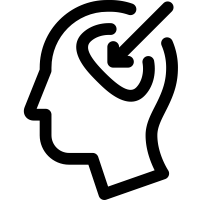
\includegraphics[width=30px]{Symbole_learn.png}}\end{minipage}
				\begin{minipage}{0.89\linewidth}\itshape\footnotesize
				}
				{                		
				\end{minipage}
			\end{minipage}\egroup;%
		\end{tikzpicture}%
	\end{center}%
}

\definecolor{colimportant}{RGB}{247 , 189 , 164}
\definecolor{contourimportant}{RGB}{237 , 125 , 49}
\newenvironment{important}
{
	\begin{center}%
		\begin{tikzpicture}%
			\node[rectangle, draw=contourimportant, top color=colimportant!50, bottom color=colimportant!140, rounded corners=5pt, inner xsep=5pt, inner ysep=6pt, outer ysep=10pt]\bgroup                     
			\begin{minipage}{0.08\linewidth}\centerline{
\includegraphics[scale=0.8]{Symbole_attention.png}}\end{minipage}
			\begin{minipage}{0.89\linewidth}
			}
			{                		
			\end{minipage}\egroup;
		\end{tikzpicture}%
	\end{center}%
}

%-----------------------------------------------------------------
%---- Modification présentation de la page: marges de la page ----
%-----------------------------------------------------------------
%\addtolength{\hoffset}{-1in}              % 1
%\addtolength{\voffset}{-1in}              % 2
\addtolength{\oddsidemargin}{-0.1 in} % 3
\addtolength{\evensidemargin}{-1in} % 3
\addtolength{\topmargin}{-1in}       % 4
\addtolength{\headheight}{6pt}       % 5
%\addtolength{\headsep}{-0.2cm}           % 6
\setlength{\textheight}{26cm}    % 7
\setlength{\textwidth}{16.5cm}      % 8
\addtolength{\marginparsep}{0pt}      % 9
\setlength{\marginparwidth}{0pt}   % 10
\addtolength{\footskip}{-1mm}           %11

\setlength{\parindent}{0em}% pas d'indentation


% Customiser le nom des sections
\usepackage{titlesec}
\titleformat{\section}[hang]{\Large \bfseries}{Série \thesection:\ }{0pt}{}

\renewcommand{\familydefault}{\sfdefault} % pour avoir des polices san serif

\newtheorem{Exc}{Exercice}
\Newassociation{correction}{Soln}{mycor}
\renewcommand{\Solnlabel}[1]{\bfseries Ex #1 }
\def\exo#1{%
	\futurelet\testchar\MaybeOptArgmyexoo}
\def\MaybeOptArgmyexoo{
	\ifx[\testchar \let\next\OptArgmyexoo
	\else \let\next\NoOptArgmyexoo \fi \next}
\def\OptArgmyexoo[#1]{%
	\begin{Exc}[#1]\normalfont}
	\def\NoOptArgmyexoo{%
		\begin{Exc}\normalfont}
		\newcommand{\finexo}{\end{Exc} \vspace{3mm}}
	\newcommand{\flag}[1]{}
	\newcommand{\entete}[1]

\newcommand{\getexocompteur}{{\the\numexpr \arabic{Exc}  \relax}}	
	
\newcommand{\eexo}{\vspace{5mm}} % espace pour séparer les exercices
\pgfplotsset{compat=1.17}
\begin{document}

\setcounter{chapter}{7}
\chapter{Programmation - Structures de contrôle}



\section{Les Boucles}
Il est souvent nécessaire en programmation de devoir répéter un bloc d'instructions un certain nombre de fois, que ce soit pour parcourir une liste, pour faire une action de manière cyclique, etc. Ce nombre d'itérations est parfois connu en avance et doit parfois être déterminé au fur et à mesure des répétitions. En fonction de la situation, il existe plusieurs structures de contrôle permettant ces répétitions. Ces structures sont appelées des \textit{boucles}.


\subsection{La boucle \textsf{for}}

\begin{defi} En python, la boucle |for| permet de répéter un bloc d'instructions pour chaque élément d'un container (tableau, chaîne de caractères, etc.). Elle est introduite par le mot-clé |for| suivi d'un nom de variable, puis du mot-clé |in| et du container à parcourir, et enfin du symbole ":" 
\end{defi}

\begin{figure}[h]\begin{center}
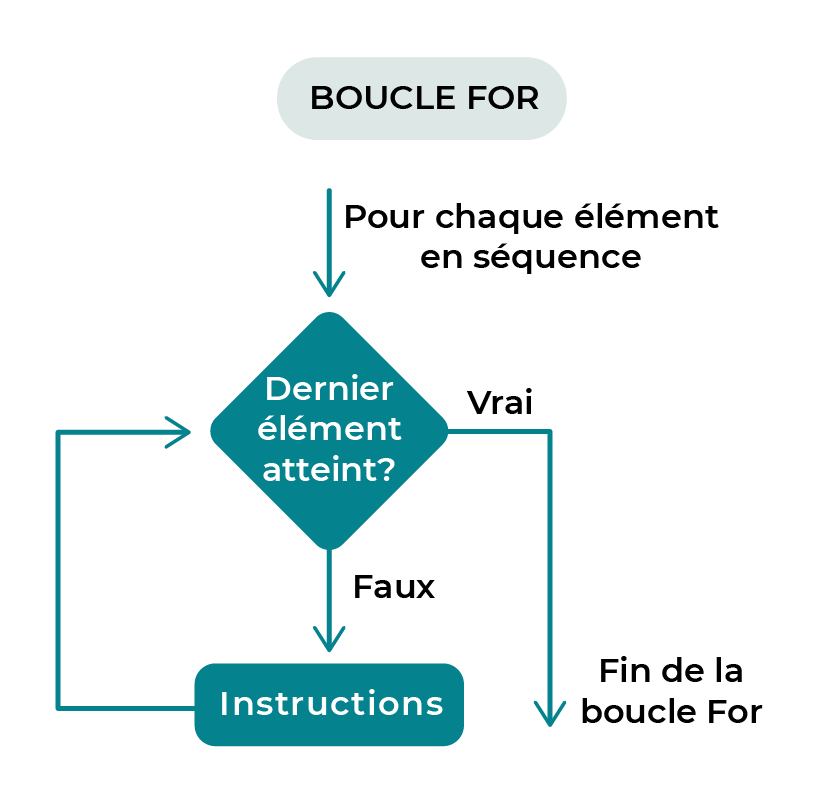
\includegraphics[scale=.3]{images/for-loop}
\caption{Schéma fonctionnel d'une boucle for}
% Source : https://openclassrooms.com/fr/courses/7168871-apprenez-les-bases-du-langage-python/7296286-repetez-des-taches-facilement-a-l-aide-de-boucles
%TODO : make smtg similar in latex 
\end{center}\end{figure}

\begin{example}
L'exemple suivant permet d'afficher 10x le mot "Coucou". À chaque itération de la boucle, le programme va exécuter la ligne contenant l'instruction |print|.
\end{example}

\lstset{caption={Boucle for - parcours tableau}}
\begin{lstlisting}
for k in range(10):
    print("Coucou")
\end{lstlisting}


\begin{remarque}
Dans les cas où l'on veut exécuter un bloc d'instructions un nombre précis de fois, la fonction |range(begin,end)| permet de générer un tableau de |begin| à |end-1| qui peut ensuite être utilisé avec une boucle |for|. L'exemple~\ref{ex:counter} peut ainsi être écrit : 

\end{remarque}

\lstset{caption={Boucle for - compteur trivial}}
\begin{lstlisting}
maxCompteur = 10
for compteur in range(maxCompteur+1):
    print(compteur)
\end{lstlisting}


\subsection{La boucle \textsf{while}}
Si la boucle |for| est la plus pratique à utiliser dans des cas précis, il existe une boucle plus modulable. C'est la boucle |while|.

\begin{defi} La boucle |while| permet de répéter un bloc d'instructions tant qu'une condition n'est pas remplie. En python, elle est introduite par le mot-clé |while| suivi d'un test terminé par le symbole ":" 
\end{defi}

\begin{figure}[h]\begin{center}
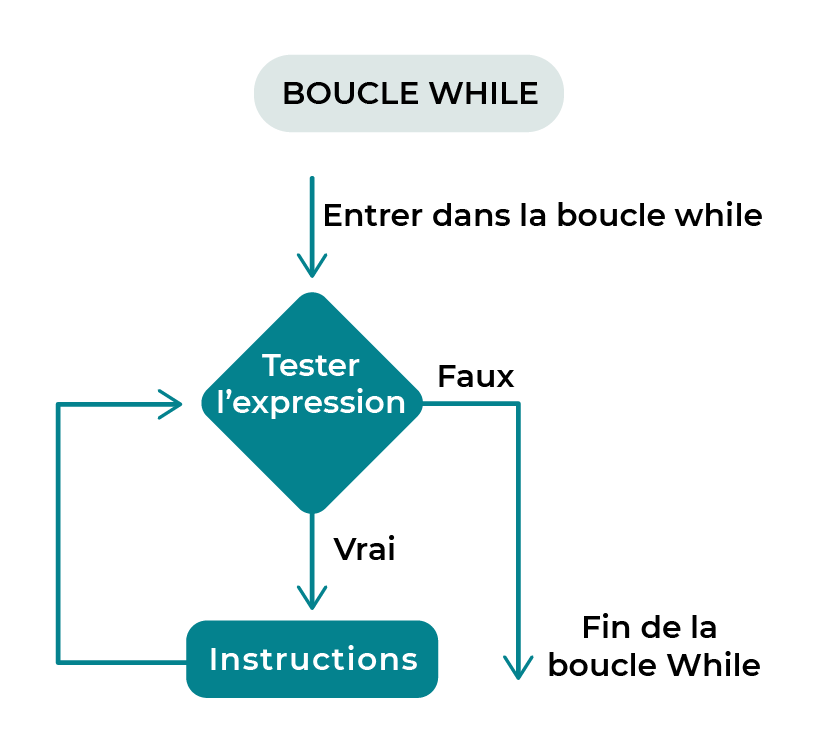
\includegraphics[scale=.3]{images/while-loop}
\caption{Schéma fonctionnel d'une boucle while}
% Source : https://openclassrooms.com/fr/courses/7168871-apprenez-les-bases-du-langage-python/7296286-repetez-des-taches-facilement-a-l-aide-de-boucles
%TODO : make smtg similar in latex 
\end{center}\end{figure}

\begin{example}
\label{ex:counter}
L'exemple suivant permet d'afficher un compteur allant de 1 à 10. À chaque début de boucle, le programme va évaluer la condition |compteur <= maxCompteur| puis exécuter le bloc d'instruction si elle vaut |True| et sortir de la boucle si elle vaut |False|.
\end{example}

\lstset{caption={Boucle while - compteur trivial}}
\begin{lstlisting}
maxCompteur = 10
compteur = 1
while compteur <= maxCompteur:
    print(compteur)
    compteur += 1
\end{lstlisting}

\begin{remarque}
L'instruction |compteur += 1| est équivalente à |compteur = compteur + 1| et sert donc à \textit{incrémenter} la variable |compteur| (à l'augmenter de 1).
\end{remarque}





\subsection{Exercices sur les ordinateurs}

\begin{exercice}
Écrire un programme listant :
\item[a)] les nombres de 0 à 50.
\item[b)] les nombres pairs de 0 à 50.
\item[a)] les nombres de 50 à 100.
\item[a)] les nombres  de 0 à 20, dans l'ordre décroissant.
\end{exercice}

\begin{exercice}
Écrire un programme qui demande à l'utilisateur-trice de saisir un nombre entier et qui affiche la table de multiplication de ce nombre de à 10.
\end{exercice}


\begin{exercice}
Calculer la somme des entiers de 1 à 100.
\end{exercice}

\begin{exercice}
Écrire un programme permettant de réaliser la figure ci-dessous :

\#\#\#\#\#\#\#\#\#\#

\#\#\#\#\#\#\#\#\#\#

\#\#\#\#\#\#\#\#\#\#

\#\#\#\#\#\#\#\#\#\#

\#\#\#\#\#\#\#\#\#\#

\#\#\#\#\#\#\#\#\#\#

\#\#\#\#\#\#\#\#\#\#

\#\#\#\#\#\#\#\#\#\#
\end{exercice}


\begin{exercice}
Écrire un programme permettant de réaliser la figure ci-dessous :

\#

\#\#

\#\#\#

\#\#\#\#

\#\#\#\#\#

\#\#\#\#\#\#

\#\#\#\#\#\#\#

\#\#\#\#\#\#\#\#

\#\#\#\#\#\#\#\#\#

\#\#\#\#\#\#\#\#\#\#
\end{exercice}


\begin{exercice}
Demander à l'utilisateur-trice de saisir un mot jusqu'à ce qu'iel saisisse un mot de plus de 5 caractères.
\end{exercice}

\begin{exercice}
Demander à l'utilisateur-trice de saisir un nombre jusqu'à ce qu'iel saisisse un nombre pair. 
\end{exercice}

\begin{exercice}
Afficher le menu d'un programme jusqu'à ce que l'utilisateur-trice saisisse "q" pour quitter.

\texttt{--- Menu --- \\
1. Option 1\\
2. Option 2\\
q. Quitter\\
Choisissez une option :}
\end{exercice}


\begin{exercice}
Écrire un programme qui demande à l'utilisateur-trice de saisir une phrase et qui affiche cette phrase sans les espaces.
\end{exercice}


\begin{exercice}
Écrire un programme qui demande à l'utilisateur-trice de saisir un mot et qui affiche ce mot à l'envers.
\end{exercice}



\begin{exercice}
Imaginer :
\item[a)] une boucle infinie, n'atteignant jamais sa condition de fin.
\item[b)] une boucle qui n'exécute jamais son bloc d'instructions.
\end{exercice}

\begin{exercice}
Écrire un programme énumérant les 100 premiers nombres de la suite de Fibonacci.
\end{exercice}

\begin{exercice}
Écrire un programme permettant d'additionner les 100 premiers entiers naturels (1, 2, ..., 100). % reponse : 5050.
\end{exercice}

\begin{exercice}
En vous inspirant de l'exercice \ref{exo:min}, écrire un programme trouvant le minimum entre N nombres.
Testez avec N=10.
\end{exercice}


%%%%%%%%%%%%%%%%%%%%%%%%%%%%%%%%%%%%%%%%%%%%%%%%%%%%%%%%%%%%%%%%%%%%%%%%%%%%%%%%%%%%%%%%%%%%%%%%%
\newpage

\section{Les conditions}

\paragraph{} Avec les concepts vus jusqu'ici, un programme exécuté 100 fois de suite donnera 100 fois les mêmes résultats, ce qui présente assez peu d'intérêt. Pour que l'exécution de notre programme dépende de différents paramètres, on utilise des structures de contrôle nommées \textit{conditions}.

\paragraph{} La condition est un élément de base d'algorithmique que l'on utilise au quotidien.
 \begin{example} S'il fait beau, j'irai en montagne. \end{example}


\paragraph{} Ces structures permettent d'exécuter ou de ne pas exécuter certaines instructions en fonction de certaines conditions et de changer ainsi le déroulement du programme.

\paragraph{}
\begin{tabular}{ c  l  }
     Étapes & Instructions \\ \hline
     1 & Se lever  \\ 
     2 & Regarder la météo  \\
     3.1 & S'il fait beau, aller en montagne  \\
\end{tabular}


\subsection{L'instruction \textsf{if}}
Un premier moyen d'exprimer des conditions en programmation est l'instruction \textsf{if}. En python, elle s'utilise de la manière suivante : 

\lstset{caption={Instruction if}}
\begin{lstlisting}
if meteo == "beau":
  print("Aujourd'hui, je vais en montagne.")
\end{lstlisting}

\begin{defi}
L'instruction |if| doit être suivie d'une expression retournant un booléen (|True| ou |False|) puis d'un symbole |:|.  Cette expression peut être une variable contenant un booléen ou une opération retournant un booléen comme les opérateurs <, >, == ou != .
\end{defi}

Dans cet exemple, si la variable |meteo| a été initialisée à |"beau"|, la phrase \textsf{Aujourd'hui, je vais en montagne.} va s'afficher. Si elle a été initialisée à une autre valeur, par exemple |meteo = "moche"|, rien ne s'affichera.

%\begin{remarque} Le début et la fin du bloc d'instructions soumis à l'instruction |if| sont définis par l'indentation de chaque ligne (le nombre d'espace avant le début du texte). La condition va s'appliquer à tout le bloc d'instruction suivant qui sera décalé vers la droite par rapport à l'instruction |if|. \end{remarque}

\begin{exercice}
Quelle est la différence entre ces deux programmes ? Qu'afficheront-ils respectivement :
\item[a)] dans le cas |meteo = "beau"| ?
\item[b)] dans le cas |meteo = "moche"| ?

\lstset{caption={Programme A}}
\begin{lstlisting}
if meteo == "beau":
  print("Aujourd'hui, ")
  print("je vais en montagne.")
\end{lstlisting}


\lstset{caption={Programme B}}
\begin{lstlisting}
if meteo == "beau":
  print("Aujourd'hui, ")
print("je vais en montagne.")
\end{lstlisting}

\end{exercice}

\paragraph{Réponse} :
\vskip+3cm



\subsection{L'instruction \textsf{else}}
L'instruction |if| peut être suivie d'une instruction |else| qui est exécutée lorsque le résultat du test est |False|. Par exemple, on pourrait préciser la situation précédente :  
 \begin{example} S'il fait beau, j'irai en montagne. Sinon, j'irai au cinéma. \end{example}
 Notre algorithme deviendrait alors : 
\paragraph{}
\begin{tabular}{ c  l  }
     Étapes & Instructions \\ \hline
     1 & Se lever  \\ 
     2 & Regarder la météo  \\
     3.1 & S'il fait beau, aller en montagne  \\
     3.2 & S'il ne fait pas beau, aller au cinéma  \\
\end{tabular}

\paragraph{}
En python, cela s'écrirait de la manière suivante :

\lstset{caption={Instruction if - else}}
\begin{lstlisting}
if meteo == "beau":
  print("Aujourd'hui, je vais en montagne.")
else:
  print("Aujourd'hui, je vais au cinéma.")
\end{lstlisting}

\subsection{L'instruction \textsf{elif}}
Dans le cas d'une situation non binaire, on peut introduire des conditions supplémentaires qui sont examinées si les conditions précédentes ne sont pas remplies. On peut par exemple nuancer notre situation ainsi : 

 \begin{example} S'il fait beau, j'irai en montagne. S'il ne fait pas beau et qu'il pleut, j'irai au cinéma. Sinon, j'irai courir au bord du Rhône. \end{example}
 
 \begin{remarque} Ici, le terme \textit{Sinon} signifie "S'il ne fait pas beau et qu'il ne pleut pas". C'est pareil en python, l'instruction conditionnée par |else| est exécutée si toutes les conditions précédentes sont fausses. \end{remarque}
 
 Notre algorithme devient alors : 
 
\paragraph{}
\begin{tabular}{ c  l  }
     Étapes & Instructions \\ \hline
     1 & Se lever  \\ 
     2 & Regarder la météo  \\
     3.1 & S'il fait beau, aller en montagne  \\
     3.2 & S'il ne fait pas beau et qu'il pleut, aller au cinéma  \\
     3.3 & S'il ne fait pas beau et qu'il pleut pas, aller courir au bord du Rhône \\
\end{tabular}

\paragraph{}
En python, on utilise l'instruction |elif| qui est la contraction de \textit{else if} :

\lstset{caption={Instruction if - else}}
\begin{lstlisting}
if meteo == "beau":
  print("Aujourd'hui, je vais en montagne.")
elif meteo == "pluie":
  print("Aujourd'hui, je vais au cinéma.")
else:
  print("Aujourd'hui, je vais courir au bord du Rhône.")
\end{lstlisting}


\subsection{Exercices sur papier}

\begin{exercice}
Que vaut la variable solution à la fin du programme suivant ? % rep : 1202
Réponse : 

\end{exercice}
\lstset{caption={Exercice}}
\begin{lstlisting}
a = True
b = ((2+2) > 4)
c = (2==3)

if c:
  solution=42
elif b:
  solution=2021
elif a:
  solution=1202
else:
  solution=73
\end{lstlisting}

\begin{exercice}
Que vaut la variable solution à la fin du programme suivant ?  % rep : C
Réponse : 
\end{exercice}

\lstset{caption={Exercice}}
\begin{lstlisting}
a = 42
b = 2021
c = 1202
d = 73

if c < (d+a):
  solution = "A"
elif b+c == a:
  solution = "B"
elif a<=42:
  solution = "C"
else:
  solution = "D"

\end{lstlisting}



\subsection{Exercices sur les ordinateurs}

\begin{exercice}
Écrivez un programme vérifiant si un nombre A est un multiple d'un autre nombre B. 
Utilisez pour cela l'opérateur modulo "\%", qui, pour |x%y|, retourne le reste de la division euclidienne de x par y. \\
Testez avec A=2941 et B=17.
\end{exercice}


\begin{exercice}
Écrivez un programme vérifiant si un nombre A est un multiple de 2 nombres B et C.\\ 
Testez avec A=26469, B=17 et C=9.
\end{exercice}


\begin{exercice}
\label{exo:min}
Écrivez un programme trouvant le minimum entre 3 nombres.
\end{exercice}

\begin{exercice}
Écrivez un programme déterminant si une année est bissextile.
\end{exercice}

%TODO
%% Joli template pour code, black skin
%% recap structure elif ?
%% exo meteo ?
%% exos prog comprendre fonctionnement complexe ?



\section{Bibliographie}
\begin{itemize}
\item  \textit{L’Informatique autrement}, De la pensée computationelle aux applications numériques, Dimitri Racordon, Damien Morard, Emmanouela Stachtiari,Aurélien Coet, Alexandre-Quentin Berger, Didier Buchs 
\item  https://openclassrooms.com/fr/courses/7168871-apprenez-les-bases-du-langage-python
\item  https://docs.python.org/fr/3/tutorial/index.html
\end{itemize}


\end{document}
